\documentclass{standalone}
\usepackage{tikz}
\usetikzlibrary{patterns}
\usetikzlibrary{positioning}
\usetikzlibrary{patterns, positioning}
\usetikzlibrary{shapes.misc}
\usepackage[outline]{contour}
\contourlength{1.5pt} 


\begin{document}
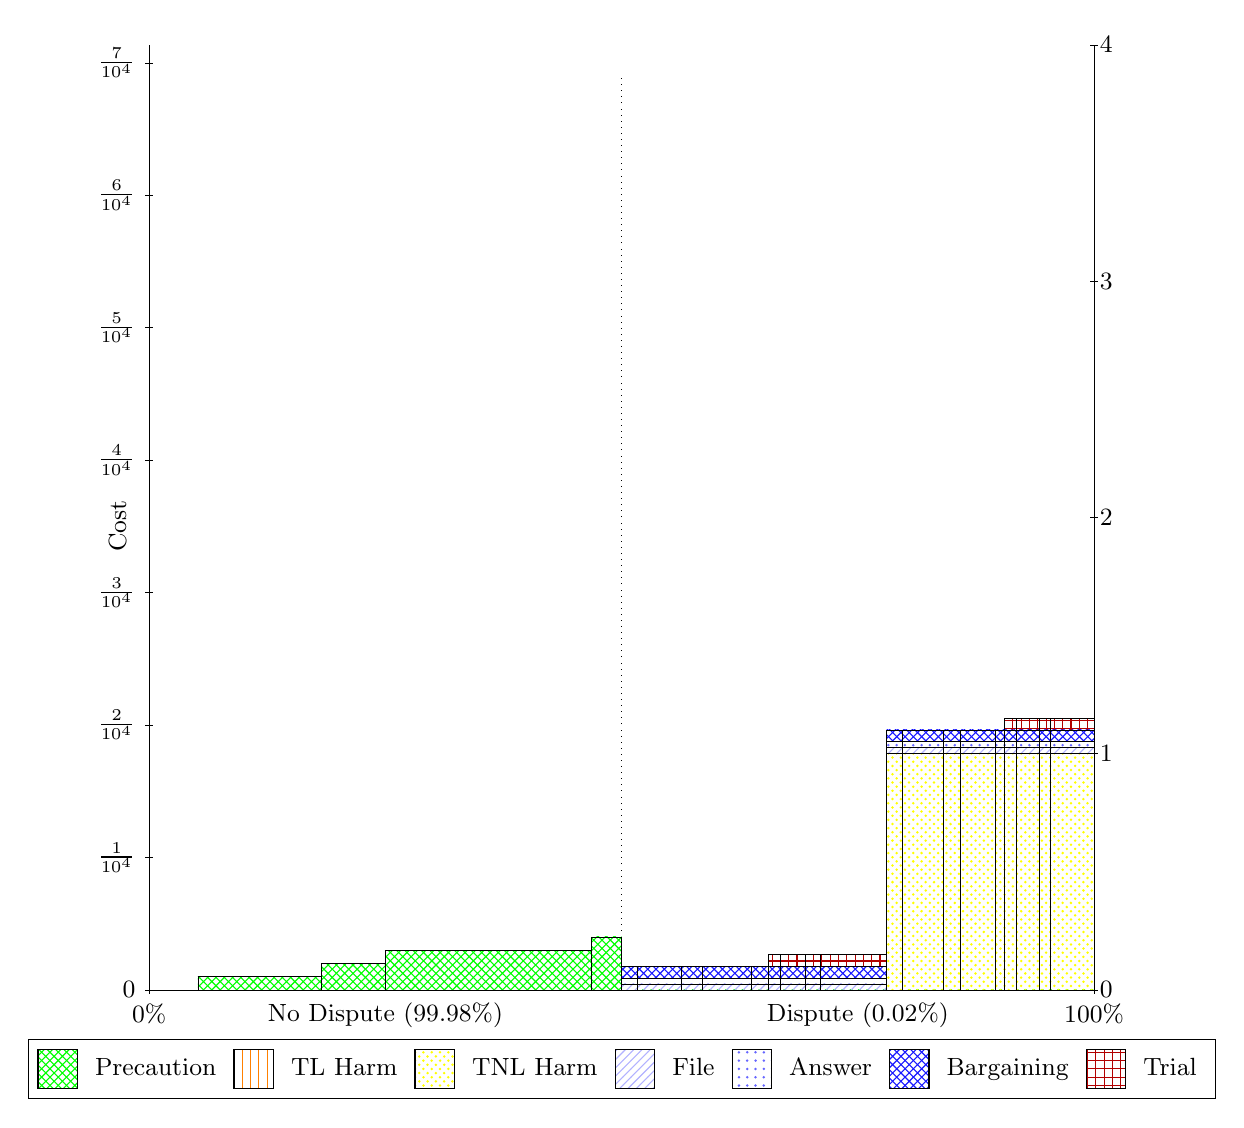
\begin{tikzpicture}
\draw[pattern=crosshatch, pattern color=green,draw=black,very thin] (2.117,2.5) rectangle (3.6907,2.6682);
\draw[pattern=crosshatch, pattern color=green,draw=black,very thin] (3.6907,2.5) rectangle (4.5,2.8364);
\draw[pattern=crosshatch, pattern color=green,draw=black,very thin] (4.5,2.5) rectangle (7.115,3.0045);
\draw[pattern=crosshatch, pattern color=green,draw=black,very thin] (7.115,2.5) rectangle (7.5,3.1727);
\draw[pattern=north east lines, pattern color=blue!30,draw=black,very thin] (7.5,2.5) rectangle (7.6963,2.575);
\draw[pattern=dots,  pattern color=blue!60,draw=black,very thin] (7.5,2.575) rectangle (7.6963,2.65);
\draw[pattern=crosshatch,      pattern color=blue!90,draw=black,very thin] (7.5,2.65) rectangle (7.6963,2.8);
\draw[pattern=crosshatch, pattern color=green,draw=black,very thin] (7.6963,2.5) rectangle (8.2545,2.5);
\draw[pattern=north east lines, pattern color=blue!30,draw=black,very thin] (7.6963,2.5) rectangle (8.2545,2.575);
\draw[pattern=dots,  pattern color=blue!60,draw=black,very thin] (7.6963,2.575) rectangle (8.2545,2.65);
\draw[pattern=crosshatch,      pattern color=blue!90,draw=black,very thin] (7.6963,2.65) rectangle (8.2545,2.8);
\draw[pattern=crosshatch, pattern color=green,draw=black,very thin] (8.2545,2.5) rectangle (8.5215,2.5001);
\draw[pattern=north east lines, pattern color=blue!30,draw=black,very thin] (8.2545,2.5001) rectangle (8.5215,2.5751);
\draw[pattern=dots,  pattern color=blue!60,draw=black,very thin] (8.2545,2.5751) rectangle (8.5215,2.6501);
\draw[pattern=crosshatch,      pattern color=blue!90,draw=black,very thin] (8.2545,2.6501) rectangle (8.5215,2.8001);
\draw[pattern=crosshatch, pattern color=green,draw=black,very thin] (8.5215,2.5) rectangle (9.1421,2.5001);
\draw[pattern=north east lines, pattern color=blue!30,draw=black,very thin] (8.5215,2.5001) rectangle (9.1421,2.5751);
\draw[pattern=dots,  pattern color=blue!60,draw=black,very thin] (8.5215,2.5751) rectangle (9.1421,2.6501);
\draw[pattern=crosshatch,      pattern color=blue!90,draw=black,very thin] (8.5215,2.6501) rectangle (9.1421,2.8001);
\draw[pattern=crosshatch, pattern color=green,draw=black,very thin] (9.1421,2.5) rectangle (9.3585,2.5001);
\draw[pattern=north east lines, pattern color=blue!30,draw=black,very thin] (9.1421,2.5001) rectangle (9.3585,2.5751);
\draw[pattern=dots,  pattern color=blue!60,draw=black,very thin] (9.1421,2.5751) rectangle (9.3585,2.6501);
\draw[pattern=crosshatch,      pattern color=blue!90,draw=black,very thin] (9.1421,2.6501) rectangle (9.3585,2.8001);
\draw[pattern=north east lines, pattern color=blue!30,draw=black,very thin] (9.3585,2.5) rectangle (9.5081,2.575);
\draw[pattern=dots,  pattern color=blue!60,draw=black,very thin] (9.3585,2.575) rectangle (9.5081,2.65);
\draw[pattern=crosshatch,      pattern color=blue!90,draw=black,very thin] (9.3585,2.65) rectangle (9.5081,2.8);
\draw[pattern=grid,            pattern color=red!70!black,draw=black,very thin] (9.3585,2.8) rectangle (9.5081,2.95);
\draw[pattern=crosshatch, pattern color=green,draw=black,very thin] (9.5081,2.5) rectangle (9.8317,2.5);
\draw[pattern=north east lines, pattern color=blue!30,draw=black,very thin] (9.5081,2.5) rectangle (9.8317,2.575);
\draw[pattern=dots,  pattern color=blue!60,draw=black,very thin] (9.5081,2.575) rectangle (9.8317,2.65);
\draw[pattern=crosshatch,      pattern color=blue!90,draw=black,very thin] (9.5081,2.65) rectangle (9.8317,2.8);
\draw[pattern=grid,            pattern color=red!70!black,draw=black,very thin] (9.5081,2.8) rectangle (9.8317,2.95);
\draw[pattern=crosshatch, pattern color=green,draw=black,very thin] (9.8317,2.5) rectangle (10.018,2.5001);
\draw[pattern=north east lines, pattern color=blue!30,draw=black,very thin] (9.8317,2.5001) rectangle (10.018,2.5751);
\draw[pattern=dots,  pattern color=blue!60,draw=black,very thin] (9.8317,2.5751) rectangle (10.018,2.6501);
\draw[pattern=crosshatch,      pattern color=blue!90,draw=black,very thin] (9.8317,2.6501) rectangle (10.018,2.8001);
\draw[pattern=grid,            pattern color=red!70!black,draw=black,very thin] (9.8317,2.8001) rectangle (10.018,2.9501);
\draw[pattern=crosshatch, pattern color=green,draw=black,very thin] (10.018,2.5) rectangle (10.866,2.5001);
\draw[pattern=north east lines, pattern color=blue!30,draw=black,very thin] (10.018,2.5001) rectangle (10.866,2.5751);
\draw[pattern=dots,  pattern color=blue!60,draw=black,very thin] (10.018,2.5751) rectangle (10.866,2.6501);
\draw[pattern=crosshatch,      pattern color=blue!90,draw=black,very thin] (10.018,2.6501) rectangle (10.866,2.8001);
\draw[pattern=grid,            pattern color=red!70!black,draw=black,very thin] (10.018,2.8001) rectangle (10.866,2.9501);
\draw[pattern=crosshatch dots, pattern color=yellow,draw=black,very thin] (10.866,2.5) rectangle (11.062,5.5);
\draw[pattern=north east lines, pattern color=blue!30,draw=black,very thin] (10.866,5.5) rectangle (11.062,5.575);
\draw[pattern=dots,  pattern color=blue!60,draw=black,very thin] (10.866,5.575) rectangle (11.062,5.65);
\draw[pattern=crosshatch,      pattern color=blue!90,draw=black,very thin] (10.866,5.65) rectangle (11.062,5.8);
\draw[pattern=crosshatch, pattern color=green,draw=black,very thin] (11.062,2.5) rectangle (11.579,2.5);
\draw[pattern=crosshatch dots, pattern color=yellow,draw=black,very thin] (11.062,2.5) rectangle (11.579,5.5);
\draw[pattern=north east lines, pattern color=blue!30,draw=black,very thin] (11.062,5.5) rectangle (11.579,5.575);
\draw[pattern=dots,  pattern color=blue!60,draw=black,very thin] (11.062,5.575) rectangle (11.579,5.65);
\draw[pattern=crosshatch,      pattern color=blue!90,draw=black,very thin] (11.062,5.65) rectangle (11.579,5.8);
\draw[pattern=crosshatch, pattern color=green,draw=black,very thin] (11.579,2.5) rectangle (11.802,2.5001);
\draw[pattern=crosshatch dots, pattern color=yellow,draw=black,very thin] (11.579,2.5001) rectangle (11.802,5.5001);
\draw[pattern=north east lines, pattern color=blue!30,draw=black,very thin] (11.579,5.5001) rectangle (11.802,5.5751);
\draw[pattern=dots,  pattern color=blue!60,draw=black,very thin] (11.579,5.5751) rectangle (11.802,5.6501);
\draw[pattern=crosshatch,      pattern color=blue!90,draw=black,very thin] (11.579,5.6501) rectangle (11.802,5.8001);
\draw[pattern=crosshatch, pattern color=green,draw=black,very thin] (11.802,2.5) rectangle (12.241,2.5001);
\draw[pattern=crosshatch dots, pattern color=yellow,draw=black,very thin] (11.802,2.5001) rectangle (12.241,5.5001);
\draw[pattern=north east lines, pattern color=blue!30,draw=black,very thin] (11.802,5.5001) rectangle (12.241,5.5751);
\draw[pattern=dots,  pattern color=blue!60,draw=black,very thin] (11.802,5.5751) rectangle (12.241,5.6501);
\draw[pattern=crosshatch,      pattern color=blue!90,draw=black,very thin] (11.802,5.6501) rectangle (12.241,5.8001);
\draw[pattern=crosshatch, pattern color=green,draw=black,very thin] (12.241,2.5) rectangle (12.359,2.5001);
\draw[pattern=crosshatch dots, pattern color=yellow,draw=black,very thin] (12.241,2.5001) rectangle (12.359,5.5001);
\draw[pattern=north east lines, pattern color=blue!30,draw=black,very thin] (12.241,5.5001) rectangle (12.359,5.5751);
\draw[pattern=dots,  pattern color=blue!60,draw=black,very thin] (12.241,5.5751) rectangle (12.359,5.6501);
\draw[pattern=crosshatch,      pattern color=blue!90,draw=black,very thin] (12.241,5.6501) rectangle (12.359,5.8001);
\draw[pattern=crosshatch dots, pattern color=yellow,draw=black,very thin] (12.359,2.5) rectangle (12.508,5.5);
\draw[pattern=north east lines, pattern color=blue!30,draw=black,very thin] (12.359,5.5) rectangle (12.508,5.575);
\draw[pattern=dots,  pattern color=blue!60,draw=black,very thin] (12.359,5.575) rectangle (12.508,5.65);
\draw[pattern=crosshatch,      pattern color=blue!90,draw=black,very thin] (12.359,5.65) rectangle (12.508,5.8);
\draw[pattern=grid,            pattern color=red!70!black,draw=black,very thin] (12.359,5.8) rectangle (12.508,5.95);
\draw[pattern=crosshatch, pattern color=green,draw=black,very thin] (12.508,2.5) rectangle (12.801,2.5);
\draw[pattern=crosshatch dots, pattern color=yellow,draw=black,very thin] (12.508,2.5) rectangle (12.801,5.5);
\draw[pattern=north east lines, pattern color=blue!30,draw=black,very thin] (12.508,5.5) rectangle (12.801,5.575);
\draw[pattern=dots,  pattern color=blue!60,draw=black,very thin] (12.508,5.575) rectangle (12.801,5.65);
\draw[pattern=crosshatch,      pattern color=blue!90,draw=black,very thin] (12.508,5.65) rectangle (12.801,5.8);
\draw[pattern=grid,            pattern color=red!70!black,draw=black,very thin] (12.508,5.8) rectangle (12.801,5.95);
\draw[pattern=crosshatch, pattern color=green,draw=black,very thin] (12.801,2.5) rectangle (12.802,2.5);
\draw[pattern=vertical lines, pattern color=orange,draw=black,very thin] (12.801,2.5) rectangle (12.802,5.5);
\draw[pattern=north east lines, pattern color=blue!30,draw=black,very thin] (12.801,5.5) rectangle (12.802,5.575);
\draw[pattern=dots,  pattern color=blue!60,draw=black,very thin] (12.801,5.575) rectangle (12.802,5.65);
\draw[pattern=crosshatch,      pattern color=blue!90,draw=black,very thin] (12.801,5.65) rectangle (12.802,5.8);
\draw[pattern=grid,            pattern color=red!70!black,draw=black,very thin] (12.801,5.8) rectangle (12.802,5.95);
\draw[pattern=crosshatch, pattern color=green,draw=black,very thin] (12.802,2.5) rectangle (12.949,2.5001);
\draw[pattern=crosshatch dots, pattern color=yellow,draw=black,very thin] (12.802,2.5001) rectangle (12.949,5.5001);
\draw[pattern=north east lines, pattern color=blue!30,draw=black,very thin] (12.802,5.5001) rectangle (12.949,5.5751);
\draw[pattern=dots,  pattern color=blue!60,draw=black,very thin] (12.802,5.5751) rectangle (12.949,5.6501);
\draw[pattern=crosshatch,      pattern color=blue!90,draw=black,very thin] (12.802,5.6501) rectangle (12.949,5.8001);
\draw[pattern=grid,            pattern color=red!70!black,draw=black,very thin] (12.802,5.8001) rectangle (12.949,5.9501);
\draw[pattern=crosshatch, pattern color=green,draw=black,very thin] (12.949,2.5) rectangle (13.5,2.5001);
\draw[pattern=crosshatch dots, pattern color=yellow,draw=black,very thin] (12.949,2.5001) rectangle (13.5,5.5001);
\draw[pattern=north east lines, pattern color=blue!30,draw=black,very thin] (12.949,5.5001) rectangle (13.5,5.5751);
\draw[pattern=dots,  pattern color=blue!60,draw=black,very thin] (12.949,5.5751) rectangle (13.5,5.6501);
\draw[pattern=crosshatch,      pattern color=blue!90,draw=black,very thin] (12.949,5.6501) rectangle (13.5,5.8001);
\draw[pattern=grid,            pattern color=red!70!black,draw=black,very thin] (12.949,5.8001) rectangle (13.5,5.9501);
\draw[black,very thin] (1.5,2.5) -- (1.5,14.5);
\node[font=\small,rotate=90,text=black, anchor=center] at (1.1, 8.3863) {Cost};
\draw[black,very thin] (1.45,2.5) -- (1.55,2.5);
\node[font=\small,text=black, anchor=east] at (1.45, 2.5) {0};
\draw[black,very thin] (1.45,4.1818) -- (1.55,4.1818);
\node[font=\small,text=black, anchor=east] at (1.45, 4.1818) {$\frac{1}{10^{4}}$};
\draw[black,very thin] (1.45,5.8636) -- (1.55,5.8636);
\node[font=\small,text=black, anchor=east] at (1.45, 5.8636) {$\frac{2}{10^{4}}$};
\draw[black,very thin] (1.45,7.5454) -- (1.55,7.5454);
\node[font=\small,text=black, anchor=east] at (1.45, 7.5454) {$\frac{3}{10^{4}}$};
\draw[black,very thin] (1.45,9.2271) -- (1.55,9.2271);
\node[font=\small,text=black, anchor=east] at (1.45, 9.2271) {$\frac{4}{10^{4}}$};
\draw[black,very thin] (1.45,10.909) -- (1.55,10.909);
\node[font=\small,text=black, anchor=east] at (1.45, 10.909) {$\frac{5}{10^{4}}$};
\draw[black,very thin] (1.45,12.591) -- (1.55,12.591);
\node[font=\small,text=black, anchor=east] at (1.45, 12.591) {$\frac{6}{10^{4}}$};
\draw[black,very thin] (1.45,14.273) -- (1.55,14.273);
\node[font=\small,text=black, anchor=east] at (1.45, 14.273) {$\frac{7}{10^{4}}$};

\draw[black,dotted,very thin] (7.5,2.86) -- (7.5,14.14);
\draw[black,very thin] (13.5,2.5) -- (13.5,14.5);
\draw[black,very thin] (13.45,2.5) -- (13.55,2.5);
\node[font=\small,text=black, anchor=west] at (13.45, 2.5) {0};
\draw[black,very thin] (13.45,5.5) -- (13.55,5.5);
\node[font=\small,text=black, anchor=west] at (13.45, 5.5) {1};
\draw[black,very thin] (13.45,8.5) -- (13.55,8.5);
\node[font=\small,text=black, anchor=west] at (13.45, 8.5) {2};
\draw[black,very thin] (13.45,11.5) -- (13.55,11.5);
\node[font=\small,text=black, anchor=west] at (13.45, 11.5) {3};
\draw[black,very thin] (13.45,14.5) -- (13.55,14.5);
\node[font=\small,text=black, anchor=west] at (13.45, 14.5) {4};

\draw[black,very thin] (1.5,2.5) -- (13.5,2.5);
\draw[black,very thin] (1.5,2.45) -- (1.5,2.55);
\node[font=\small,text=black, anchor=north] at (1.5, 2.45) {0\%};
\draw[black,very thin] (13.5,2.45) -- (13.5,2.55);
\node[font=\small,text=black, anchor=north] at (13.5, 2.45) {100\%};

\node[font=\small,text=black,anchor=south] at (4.5, 1.9) {No\ Dispute\ (99.98\%)};
\node[font=\small,text=black,anchor=south] at (10.5, 1.9) {Dispute\ (0.02\%)};
\draw (7.5,2.5) node (B) {};
\begin{scope}[align=center]
\matrix[scale=0.5,draw=black,below=0.5cm of B,nodes={draw},column sep=0.1cm]{
\node[rectangle,draw,minimum width=0.5cm,minimum height=0.5cm,pattern=crosshatch, pattern color=green]{}; & \node[draw=none,font=\small,text=black]{Precaution}; &
\node[rectangle,draw,minimum width=0.5cm,minimum height=0.5cm,pattern=vertical lines, pattern color=orange]{}; & \node[draw=none,font=\small,text=black]{TL Harm}; &
\node[rectangle,draw,minimum width=0.5cm,minimum height=0.5cm,pattern=crosshatch dots, pattern color=yellow]{}; & \node[draw=none,font=\small,text=black]{TNL Harm}; &
\node[rectangle,draw,minimum width=0.5cm,minimum height=0.5cm,pattern=north east lines, pattern color=blue!30]{}; & \node[draw=none,font=\small,text=black]{File}; &
\node[rectangle,draw,minimum width=0.5cm,minimum height=0.5cm,pattern=dots,  pattern color=blue!60]{}; & \node[draw=none,font=\small,text=black]{Answer}; &
\node[rectangle,draw,minimum width=0.5cm,minimum height=0.5cm,pattern=crosshatch,      pattern color=blue!90]{}; & \node[draw=none,font=\small,text=black]{Bargaining}; &
\node[rectangle,draw,minimum width=0.5cm,minimum height=0.5cm,pattern=grid,            pattern color=red!70!black]{}; & \node[draw=none,font=\small,text=black]{Trial}; \\\\
};\end{scope}

\end{tikzpicture}
\end{document}